\documentclass[journal,a4paper]{IEEEtran}
\usepackage[utf8]{inputenc}
\usepackage[T1]{fontenc}
\usepackage[spanish,es-noshorthands,es-tabla]{babel}
\usepackage{amsmath,amssymb}
\usepackage{icomma}
\usepackage{graphicx}
\usepackage{booktabs}
\usepackage{array}
\usepackage{xcolor}
\usepackage{tikz}
\usetikzlibrary{arrows.meta,positioning}
\usepackage{pgfplots}
\pgfplotsset{compat=1.18}
\usepackage[european]{circuitikz}
\usepackage[hidelinks]{hyperref}

\graphicspath{{figuras/bn/}{figuras/}}
\pgfplotsset{every axis/.append style={
  grid=both, major grid style={gray!45}, minor grid style={gray!15},
  tick label style={font=\footnotesize}, label style={font=\footnotesize},
  legend style={font=\scriptsize}, /pgf/number format/use comma}}

\begin{document}

\title{Amplificador de instrumentación para la adquisición de señales de ECG}

\author{Ernst Pedro (Leg. 400624), Polizze Tomás (Leg. 400793), Rao Valentino (Leg. 402308)\\
\textit{Electrónica Aplicada 2 4R2, Ingeniería Electrónica, Facultad Regional Córdoba}\\
\textit{Universidad Tecnológica Nacional}}

\maketitle

\begin{abstract}
En este informe se pone a punto y se caracteriza experimentalmente un amplificador de entrada diferencial para señales de electrocardiograma (ECG). El circuito está formado por un amplificador de instrumentación de tres amplificadores operacionales con un filtro pasabanda integrado en el restador, seguido de una etapa de ganancia ajustable. El circuito se simuló en LTspice y luego se caracterizó en el laboratorio: se midió una ganancia diferencial de 60,3\,dB, una frecuencia de corte superior de 116\,Hz y una relación de rechazo de modo común (RRMC) de 97,2\,dB a 50\,Hz, que cumplen las especificaciones de diseño. Por último, se validó el sistema con un simulador de señales biológicas y se obtuvo un trazado P-QRS-T limpio de 1,08\,Vpp a partir de una señal de 1\,mVpp.
\end{abstract}

\begin{IEEEkeywords}
Amplificador de instrumentación, ECG, RRMC, modo común, respuesta en frecuencia, filtro pasabanda, TL084.
\end{IEEEkeywords}

%======================================================================
\section{Introducción}

\IEEEPARstart{L}{a} señal de ECG que se capta sobre la superficie del cuerpo tiene una amplitud del orden de 1\,mV y su contenido espectral útil se concentra entre unas centésimas de hertz y algo más de 100\,Hz. Sobre esa señal diferencial se monta una tensión de modo común, inducida principalmente por la red eléctrica de 50\,Hz, que puede ser varios órdenes de magnitud mayor. Por eso el amplificador de entrada tiene que amplificar la diferencia entre dos electrodos y, al mismo tiempo, rechazar lo que es común a ambos.

Para este trabajo se utiliza la derivación~I de Einthoven: la entrada no inversora se conecta al brazo izquierdo (LA), la inversora al brazo derecho (RA) y la pierna derecha (RL) se usa como referencia. Las especificaciones de diseño se resumen en la Tabla~\ref{tab:specs}.

\begin{table}[!h]
\centering
\caption{Especificaciones de diseño}
\label{tab:specs}
\begin{tabular}{@{}ll@{}}
\toprule
Parámetro & Valor \\ \midrule
Ganancia diferencial $A_{md}$ & 60\,dB (1000\,V/V) \\
Frecuencia de corte inferior $f_L$ & 0,05\,Hz \\
Frecuencia de corte superior $f_H$ & 100\,Hz \\
RRMC & $\gg 80$\,dB \\
Impedancia de entrada $Z_i$ & $> 5$\,M$\Omega$ \\
Amplitud de la señal de entrada & 1\,mVpp \\ \bottomrule
\end{tabular}
\end{table}

%======================================================================
\section{Descripción del circuito}

El diagrama en bloques del sistema se muestra en la Fig.~\ref{fig:bloques}, y el esquemático del camino de la señal en la Fig.~\ref{fig:esquematico}. Se utiliza un único TL084, cuádruple con entrada JFET: su impedancia de entrada del orden de $10^{12}\,\Omega$ y su corriente de polarización de decenas de pA evitan cargar la interfaz electrodo-piel. El offset relativamente alto (hasta algunos mV) no es un problema, porque la segunda etapa está acoplada en alterna.

\begin{figure}[!t]
\centering
\begin{tikzpicture}[
  blk/.style={draw, rounded corners=2pt, align=center, minimum height=1.05cm, font=\footnotesize, text width=1.7cm},
  >={Stealth[length=2mm]}, node distance=0.4cm]
\node[font=\footnotesize, align=center] (in) {LA\\RA\\RL};
\node[blk, right=0.35cm of in] (ai) {Amp. de\\instrumentación\\$G_1=100{,}8$};
\node[blk, right=of ai] (bp) {Restador\\pasabanda\\0,048--106\,Hz};
\node[blk, right=of bp] (g3) {Inversor\\$G_3\approx 10$\\(RV2)};
\node[font=\footnotesize, right=0.3cm of g3] (out) {$v_o$};
\draw[->] (in) -- (ai);
\draw[->] (ai) -- (bp);
\draw[->] (bp) -- (g3);
\draw[->] (g3) -- (out);
\end{tikzpicture}
\caption{Diagrama en bloques del amplificador de ECG.}
\label{fig:bloques}
\end{figure}

\begin{figure}[!t]
\centering
\resizebox{\columnwidth}{!}{% Camino de senal del amplificador de ECG, dibujado para una columna IEEE.
\begin{circuitikz}[font=\footnotesize]
\ctikzset{bipoles/length=0.85cm, amplifiers/scale=0.62, diodes/scale=0.5,
  resistors/scale=0.7, capacitors/scale=0.6, grounds/scale=0.6}
\tikzset{dot/.style={circle, fill, inner sep=0pt, minimum size=2.6pt}}
% ---------------- Etapa 1: amplificador de instrumentacion ----------------
\node[op amp, noinv input up] (B) at (3.0,3.0) {};
\node[op amp] (A) at (3.0,0.2) {};
\node at (3.25,3.6) {U1B};
\node at (3.25,-0.4) {U1A};
% entrada + (LA): R1 y diodos D1/D3 a masa
\draw (0,0 |- B.+) node[ocirc] (la) {} to[R, l=$R_1$, a=10k] (0.85,0 |- B.+)
  -- (B.+);
\node[left] at (la) {LA};
\draw (1.0,0 |- B.+) node[dot] {} to[D] ++(0,-0.55) node[ground] {};
\draw (1.27,0 |- B.+) node[dot] {} to[D, invert] ++(0,-0.55) node[ground] {};
% entrada - (RA): R2 y diodos D2/D4 a masa
\draw (0,0 |- A.+) node[ocirc] (ra) {} to[R, l_=$R_2$, a^=10k] (0.85,0 |- A.+)
  -- (A.+);
\node[left] at (ra) {RA};
\draw (1.0,0 |- A.+) node[dot] {} to[D] ++(0,-0.55) node[ground] {};
\draw (1.27,0 |- A.+) node[dot] {} to[D, invert] ++(0,-0.55) node[ground] {};
% R3 entre las entradas inversoras
\draw (B.-) -- (1.7,0 |- B.-) node[dot] {} to[R, l_={$R_3$ 10k}] (1.7,0 |- A.-) node[dot] {} -- (A.-);
% realimentaciones R5 y R4
\draw (1.95,0 |- B.-) node[dot] {} |- (2.25,2.05) to[R, l={$R_5$ 499k}] (3.4,2.05) -| (3.95,0 |- B.out) -- (B.out);
\draw (1.95,0 |- A.-) node[dot] {} |- (2.25,1.15) to[R, l_={$R_4$ 499k}] (3.4,1.15) -| (3.95,0 |- A.out) -- (A.out);
% ---------------- Etapa 2: restador con filtro pasabanda ----------------
\node[op amp] (C) at (6.95,1.6) {};
\node at (7.25,1.0) {U1C};
\draw (3.95,0 |- B.out) node[dot] {} to[R, l=$R_6$, a=100k] (4.85,0 |- B.out)
  to[C, l=$C_3$, a=33$\mu$] (5.6,0 |- B.out) |- (C.-);
\draw (3.95,0 |- A.out) node[dot] {} to[R, l_=$R_7$, a^=100k] (4.85,0 |- A.out)
  to[C, l_=$C_4$, a^=33$\mu$] (5.6,0 |- A.out) |- (C.+);
% realimentacion R10 || C7
\draw (5.85,0 |- C.-) node[dot] {} -- (5.85,3.3) node[dot] {} to[R, l_={$R_{10}$ 100k}] (7.95,3.3) node[dot] {}
  -- (7.95,0 |- C.out) node[dot] {} -- (C.out);
\draw (5.85,3.3) -- (5.85,4.0) to[C, l={$C_7$ 15n}] (7.95,4.0) -- (7.95,3.3);
% rama a masa de la entrada +: C8 y R8 + R9 + RV1
\draw (5.85,0 |- C.+) node[dot] {} -- (5.85,-0.15) node[dot] {} to[C, l={$C_8$ 15n}] (5.85,-0.95) node[ground] {};
\draw (5.85,-0.15) -- (7.25,-0.15) to[R, l={$R_8{+}R_9$ 98k}] (7.25,-1.05) to[vR, l={RV1 5k}] (7.25,-1.95) node[ground] {};
% ---------------- Etapa 3: inversor de salida ----------------
\node[op amp, anchor=-] (D) at (10.01,1.6) {};
\node at (11.05,0.68) {U1D};
\draw (7.95,0 |- C.out) to[R, l=$R_{11}$, a={4,7k}] (8.95,0 |- C.out)
  to[vR, l=RV2, a=10k] (9.8,0 |- C.out) node[dot] {} -- (D.-);
\draw (D.+) -- (9.8,0 |- D.+) node[ground] {};
\draw (9.8,0 |- C.out) -- (9.8,2.45) to[R, l={$R_{12}$ 100k}] (11.7,2.45) -- (11.7,0 |- D.out) node[dot] {} -- (D.out);
\draw (11.7,0 |- D.out) -- (12.0,0 |- D.out) node[ocirc] (vo) {};
\node[right] at (vo) {$v_o$};
\end{circuitikz}
}
\caption{Esquemático del camino de la señal. U1A/U1B forman la etapa de entrada del amplificador de instrumentación, U1C el restador con filtro pasabanda y U1D la etapa de salida. No se muestran la alimentación ($\pm 15$\,V, desacoplada con C1, C2, C5 y C6) ni los conectores.}
\label{fig:esquematico}
\end{figure}

\subsection{Protección de entrada}
Cada entrada pasa por una resistencia serie de 10\,k$\Omega$ (R1, R2) y un par de diodos 1N4148 en antiparalelo a masa (D1--D4), que recortan cualquier tensión que supere unos $\pm 0{,}6$\,V. Con esto se protegen las entradas del operacional sin afectar la señal de ECG, que es de algunos mV.

\subsection{Etapa de entrada (U1A, U1B)}
Los dos seguidores con ganancia comparten la resistencia R3 y forman la primera etapa del amplificador de instrumentación. Su ganancia diferencial es
\begin{equation}
G_1 = 1 + \frac{2R_4}{R_3} = 1 + \frac{2\cdot 499\,\text{k}\Omega}{10\,\text{k}\Omega} = 100{,}8,
\end{equation}
mientras que el modo común pasa con ganancia unitaria. Al estar las entradas sobre las patas no inversoras, la impedancia de entrada queda determinada por el TL084 y supera ampliamente los 5\,M$\Omega$ requeridos.

\subsection{Restador con filtro pasabanda (U1C)}
El restador recibe las dos salidas de la primera etapa a través de las impedancias $Z_3 = R_6 + 1/(sC_3)$ y realimenta con $Z_4 = R_{10}\parallel 1/(sC_7)$. La rama no inversora está duplicada (R7, C4, C8) y su resistencia a masa está formada por R8 + R9 + RV1 (98 a 103\,k$\Omega$), de modo que el trimmer RV1 permite balancear el puente y maximizar la RRMC. Con $R_6 = R_{10} = R$, la transferencia de la etapa es
\begin{equation}
H_2(s) = \frac{Z_4}{Z_3} = \frac{sRC_3}{(1+sRC_3)(1+sRC_7)},
\end{equation}
con ganancia unitaria en la banda de paso. El cero en el origen y el polo en $1/(RC_3)$ dan el acoplamiento en alterna, que bloquea los offsets de la primera etapa y la deriva de los electrodos. El polo en $1/(RC_7)$ limita el ancho de banda superior:
\begin{align}
f_L &= \frac{1}{2\pi R C_3} = \frac{1}{2\pi\cdot 100\,\text{k}\Omega\cdot 33\,\mu\text{F}} = 0{,}048\,\text{Hz},\\
f_H &= \frac{1}{2\pi R C_7} = \frac{1}{2\pi\cdot 100\,\text{k}\Omega\cdot 15\,\text{nF}} = 106\,\text{Hz}.
\end{align}

\subsection{Etapa de salida (U1D)}
Es un amplificador inversor con
\begin{equation}
G_3 = -\frac{R_{12}}{R_{11}+R_{V2}} = -\frac{100\,\text{k}\Omega}{4{,}7\,\text{k}\Omega + R_{V2}},
\end{equation}
ajustable entre $-6{,}8$ y $-21{,}3$. Para una ganancia total de 1000 se necesita $|G_3| = 1000/100{,}8 = 9{,}92$, es decir $R_{V2}\approx 5{,}4$\,k$\Omega$. Como el restador invierte la señal y esta etapa la vuelve a invertir, la salida queda en fase con la entrada no inversora. La ganancia total en la banda de paso resulta
\begin{equation}
A_{md} = G_1\,|H_2|\,|G_3| \approx 100{,}8 \cdot 1 \cdot 9{,}92 = 1000 \;(60\,\text{dB}).
\end{equation}

%======================================================================
\section{Diseño de la placa}

El circuito impreso se diseñó en KiCad a partir del esquemático de la Fig.~\ref{fig:esquematico}. Se eligió una placa \textbf{simple faz} de 100\,$\times$\,50\,mm, con todo el cobre en la cara inferior y sin vías ni puentes, para poder fabricarla en forma casera por transferencia térmica de tóner (planchado). Por el mismo motivo se usaron pistas anchas, de 0,75\,mm, y una aislación mínima de 0,6\,mm, que toleran las imperfecciones de ese proceso. El área libre de la cara de cobre se rellenó con un plano de masa, que reduce la impedancia del retorno común y ayuda a blindar los nodos de alta impedancia frente al acoplamiento de la red. La Fig.~\ref{fig:placa} muestra la vista 3D del lado de componentes y la capa de cobre.

La distribución sigue el flujo de la señal de izquierda a derecha:
\begin{itemize}
\item en el borde izquierdo están las borneras de entrada (J1: LA, RA y RL) y de alimentación (J3), junto con los electrolíticos de filtrado C1 y C2;
\item a continuación, el conector J2 con un jumper permite unir la entrada inversora a masa (ensayos diferenciales) o unir ambas entradas (ensayos de modo común) sin recablear;
\item las resistencias serie y los diodos de protección de las dos entradas están dispuestos en forma simétrica, antes de la etapa de entrada;
\item el TL084 va montado en un zócalo DIP-14 en el centro de la placa, y lo rodean las redes de las tres etapas;
\item los dos trimmers multivuelta (RV1 y RV2, Bourns 3296W) están del lado derecho, accesibles para el ajuste, y la salida se toma de los pines J4 y J5.
\end{itemize}
Los capacitores de desacople C5 y C6 (100\,nF) son SMD 0805 y van soldados del lado del cobre, directamente junto a los pines de alimentación del integrado (4 y 11). El resto de los componentes es de inserción. La lista completa se detalla en la Tabla~\ref{tab:bom}.

\begin{figure}[!t]
\centering
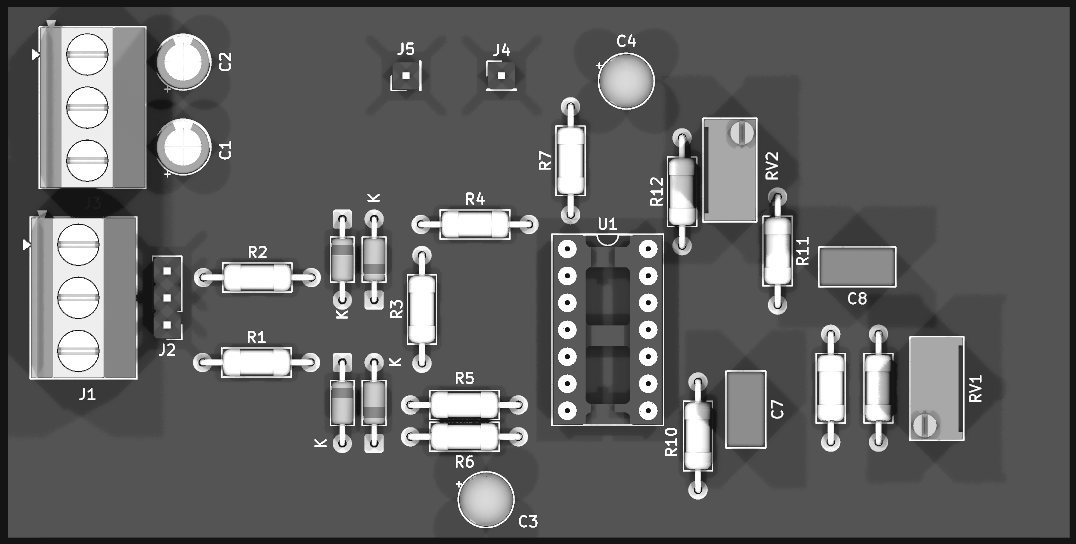
\includegraphics[width=\columnwidth]{placa_3d.jpg}\\[-1pt]
{\footnotesize (a) Vista 3D del lado de componentes}\\[5pt]
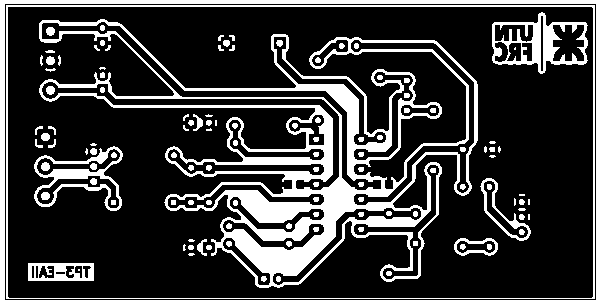
\includegraphics[width=\columnwidth]{placa_cobre.pdf}\\[-1pt]
{\footnotesize (b) Capa de cobre (cara inferior, vista desde arriba)}
\caption{Diseño del circuito impreso, 100\,$\times$\,50\,mm, simple faz.}
\label{fig:placa}
\end{figure}

\begin{table}[!t]
\centering
\caption{Lista de componentes}
\label{tab:bom}
\footnotesize
\begin{tabular}{@{}lll@{}}
\toprule
Designador & Valor & Encapsulado \\ \midrule
R1, R2, R3 & 10\,k$\Omega$ & Axial 1/4\,W \\
R4, R5 & 499\,k$\Omega$ & Axial 1/4\,W \\
R6, R7, R10, R12 & 100\,k$\Omega$ & Axial 1/4\,W \\
R8 & 47\,k$\Omega$ & Axial 1/4\,W \\
R9 & 51\,k$\Omega$ & Axial 1/4\,W \\
R11 & 4,7\,k$\Omega$ & Axial 1/4\,W \\
RV1 & 5\,k$\Omega$ & Trimmer 3296W \\
RV2 & 10\,k$\Omega$ & Trimmer 3296W \\
C1, C2 & 47\,$\mu$F & Electrolítico radial \\
C3, C4 & 33\,$\mu$F & Electrolítico radial \\
C5, C6 & 100\,nF & Cerámico SMD 0805 \\
C7, C8 & 15\,nF & Poliéster \\
D1--D4 & 1N4148 & DO-35 \\
U1 & TL084 & DIP-14 en zócalo \\
J1, J3 & Bornera 3 vías & Paso 5\,mm \\
J2 & Pines 1$\times$3 + jumper & Paso 2,54\,mm \\
J4, J5 & Pin & Paso 2,54\,mm \\ \bottomrule
\end{tabular}
\end{table}

%======================================================================
\section{Simulación en LTspice}

Antes de comparar con las mediciones, se simuló el circuito completo en LTspice. El esquemático de LTspice reproduce la placa componente por componente, con el modelo macro ADTL084 de Analog Devices para cada sección del TL084, el modelo del 1N4148 para los diodos de protección y la misma alimentación de $\pm 15$\,V usada en el laboratorio. Los trimmers se fijaron en sus valores nominales: $R_{V1} = 2$\,k$\Omega$, que balancea exactamente el restador ($R_8+R_9+R_{V1} = R_{10}$), y $R_{V2} = 5{,}38$\,k$\Omega$, que da la ganancia de diseño. Se realizaron tres análisis:
\begin{itemize}
\item \textbf{AC diferencial}: señal en la entrada no inversora y entrada inversora a masa, entre 1\,mHz y 10\,kHz;
\item \textbf{AC de modo común}: ambas entradas unidas, con C8 desbalanceado respecto de C7 en 0, 0,63, 2 y 5\,\%;
\item \textbf{Transitorio}: senoidal de 10\,mVpp a 25\,Hz en modo diferencial.
\end{itemize}

Los resultados principales se resumen en la Tabla~\ref{tab:sim}. Las frecuencias de corte simuladas coinciden con las calculadas en la sección anterior, y la ganancia de la primera etapa es de 40,06\,dB (100,7\,V/V). La ganancia máxima es levemente menor que 60\,dB porque a 25\,Hz el polo de 106\,Hz ya resta 0,23\,dB. La Fig.~\ref{fig:tran} muestra las formas de onda del transitorio: las salidas de la primera etapa están en contrafase y tienen casi la misma amplitud, y la salida final está en fase con la entrada.

\begin{table}[!t]
\centering
\caption{Resultados de la simulación}
\label{tab:sim}
\begin{tabular}{@{}lr@{}}
\toprule
Magnitud & Valor simulado \\ \midrule
Ganancia máxima $A_{md}$ & 59,98\,dB (997\,V/V) \\
Ganancia a 25\,Hz & 59,75\,dB (972\,V/V) \\
$f_L$ & 0,0482\,Hz \\
$f_H$ & 106,2\,Hz \\ \midrule
\multicolumn{2}{@{}l}{Transitorio, $V_{in} = 10$\,mVpp a 25\,Hz:} \\
\quad $V_{pin1}$ / $V_{pin7}$ & 498 / 508\,mVpp \\
\quad $V_{pin8}$ & 980\,mVpp \\
\quad $V_{out}$ & 9,72\,Vpp \\ \bottomrule
\end{tabular}
\end{table}

\begin{figure}[!t]
\centering
\begin{tikzpicture}
\begin{axis}[
  width=\columnwidth, height=3.7cm, xmin=120, xmax=200,
  ylabel={Tensión (mV)}, xticklabels={}, ymin=-330, ymax=330,
  legend columns=3, legend style={at={(0.5,1.03)}, anchor=south}]
\addplot[black, thick] table[x=t, y expr=\thisrow{v7}*1000] {datos/sim_tran_25hz.dat};
\addlegendentry{pin 7}
\addplot[black, dashed, thick] table[x=t, y expr=\thisrow{v1}*1000] {datos/sim_tran_25hz.dat};
\addlegendentry{pin 1}
\addplot[gray, thick] table[x=t, y expr=\thisrow{vin}*10] {datos/sim_tran_25hz.dat};
\addlegendentry{$v_{in}\times 10$}
\end{axis}
\end{tikzpicture}\\[-2pt]
\begin{tikzpicture}
\begin{axis}[
  width=\columnwidth, height=3.7cm, xmin=120, xmax=200,
  xlabel={$t$ (ms)}, ylabel={Tensión (V)}, ymin=-6, ymax=6,
  legend columns=2, legend style={at={(0.5,0.97)}, anchor=north, fill=white}]
\addplot[black, thick] table[x=t, y=vout] {datos/sim_tran_25hz.dat};
\addlegendentry{salida (pin 14)}
\addplot[black, dashed, thick] table[x=t, y expr=\thisrow{v8}*5] {datos/sim_tran_25hz.dat};
\addlegendentry{pin 8 $\times 5$}
\end{axis}
\end{tikzpicture}
\caption{Transitorio simulado con 10\,mVpp a 25\,Hz. Arriba, la entrada y las salidas de la primera etapa. Abajo, la salida del restador (pin 8, escalada) y la salida final.}
\label{fig:tran}
\end{figure}

En modo común, con todos los componentes ideales, el restador queda perfectamente balanceado y la ganancia de modo común a 50\,Hz es de apenas $-133$\,dB. En un circuito real ese valor no se alcanza, porque el apareamiento de las dos ramas del restador nunca es perfecto. Con RV1 en el balance resistivo exacto, el desbalance que queda proviene de C7 y C8. Para un apartamiento relativo $\delta$ entre ambos capacitores, el análisis del restador da
\begin{equation}
A_{mc} \approx |G_3|\,\frac{1}{2}\,\frac{\omega R C_7\,\delta}{\sqrt{1+(\omega R C_7)^2}},
\end{equation}
que crece con la frecuencia. La simulación con distintos valores de $\delta$ se compara con las mediciones en la Sección~\ref{sec:rrmc}.

%======================================================================
\section{Puesta a punto de la placa}

En la primera prueba con señal, la salida del pin~1 (U1A) saturaba de riel a riel con una onda cuadrada de unos 25\,Vpp, mientras que el pin~7 (U1B) reproducía la entrada con ganancia unitaria. Ese comportamiento corresponde a la realimentación de U1A abierta: sin corriente por R4 tampoco circula corriente por R3, U1B queda como seguidor y U1A trabaja a lazo abierto como comparador. La causa era un pad sin soldar en el nodo que une el pin~1 con R4 y R7. Una vez resoldado, la primera etapa respondió con la ganancia esperada.

Con la primera etapa funcionando, la ganancia entre su salida diferencial y la salida final daba $\approx 2$ en lugar de $\approx 10$. Al revisar la etapa de salida se encontró que R11 era de 47\,k$\Omega$ en lugar de 4,7\,k$\Omega$ (los dos valores solo difieren en la banda multiplicadora). Se reemplazó por el valor correcto.

La placa se alimentó con la fuente fija de $\pm 15$\,V del laboratorio, en lugar de los $\pm 12$\,V de diseño. Esto no modifica las ganancias y solo amplía la excursión de salida a unos $\pm 13{,}5$\,V.

%======================================================================
\section{Instrumental y método}

Se utilizó un osciloscopio Rigol DS1052E y un generador de funciones UNI-T UTG1042X con la carga configurada en alta impedancia. El generador se conectó directamente a la placa, sin divisor resistivo, ajustando la amplitud en el propio generador: $\approx 10$\,mVpp para los ensayos diferenciales y $\approx 520$\,mVpp para los de modo común. Para los ensayos diferenciales, la entrada inversora se puso a masa con el jumper de la placa. Para los de modo común, ambas entradas se unieron entre sí.

Medir directamente una señal de 10\,mVpp resultó poco confiable. Con CH1 en 20\,mV/div la señal ocupaba apenas media división, y la lectura de Vpp quedaba dominada por el ruido. Para estimar la amplitud real de entrada se usaron dos métodos:
\begin{itemize}
\item medición en CH1 con adquisición promediada (64 muestras), que dio $V_{in} = 11{,}2$\,mVpp;
\item cálculo a partir de la primera etapa, cuya ganancia la fijan resistencias al 1\,\%: $V_{in} = (V_{pin1}+V_{pin7})/G_1 = (484+492)\,\text{mV}/100{,}8 = 9{,}68$\,mVpp.
\end{itemize}

También se comprobó que el filtro digital del osciloscopio atenuaba las lecturas entre 100 y 500\,Hz. Los puntos medidos con ese filtro se descartaron y se repitieron con el filtro desactivado, usando adquisición promediada.

%======================================================================
\section{Ganancia diferencial}

Con una señal senoidal de 25\,Hz se ajustó RV2 para llevar la ganancia total al valor de diseño. Los resultados se resumen en la Tabla~\ref{tab:amd}. Según cuál de las dos estimaciones de $V_{in}$ se tome, la ganancia queda entre 964 y 1116, es decir entre 59,7 y 61,0\,dB. Se adopta el valor medio, $A_{md}\approx 1040$ (60,3\,dB), que coincide con la ganancia de 1048 obtenida a 25\,Hz en el barrido en frecuencia. Las salidas de la primera etapa son prácticamente iguales en amplitud (484 y 492\,mVpp) y están en contrafase, lo que confirma el balance de U1A/U1B.

\begin{table}[!t]
\centering
\caption{Ganancia diferencial a 25\,Hz}
\label{tab:amd}
\begin{tabular}{@{}lr@{}}
\toprule
Magnitud & Valor \\ \midrule
$V_{in}$ medida (promediada) & 11,2\,mVpp \\
$V_{pin1}$ / $V_{pin7}$ & 484 / 492\,mVpp \\
$V_{in}$ calculada con la etapa 1 & 9,68\,mVpp \\
$V_{out}$ & 10,8\,Vpp \\ \midrule
$A_{md}$ con $V_{in}$ medida & 964 (59,7\,dB) \\
$A_{md}$ con $V_{in}$ calculada & 1116 (61,0\,dB) \\
$A_{md}$ adoptada & \textbf{1040 (60,3\,dB)} \\ \bottomrule
\end{tabular}
\end{table}

%======================================================================
\section{Respuesta en frecuencia}

Se barrió la frecuencia entre 1\,Hz y 2\,kHz, con la amplitud del generador fija y sin tocar RV2. Como la lectura directa de la entrada era ruidosa, la ganancia se calculó con un valor constante $V_{in} = 10{,}4$\,mVpp, el medido a 25\,Hz. La Tabla~\ref{tab:barrido} muestra los resultados y la Fig.~\ref{fig:bode} los compara con la simulación.

\begin{table}[!t]
\centering
\caption{Respuesta en frecuencia ($V_{in} = 10{,}4$\,mVpp)}
\label{tab:barrido}
\begin{tabular}{@{}rrrr@{}}
\toprule
$f$ (Hz) & $V_{out}$ (Vpp) & $G$ (V/V) & $G$ (dB) \\ \midrule
1 & 11,4 & 1096 & 60,8 \\
5 & 11,2 & 1077 & 60,6 \\
10 & 11,1 & 1067 & 60,6 \\
25 & 10,9 & 1048 & 60,4 \\
50 & 10,0 & 962 & 59,7 \\
75 & 9,04 & 869 & 58,8 \\
98,8 & 8,72 & 838 & 58,5 \\
125 & 7,76 & 746 & 57,5 \\
150 & 7,04 & 677 & 56,6 \\
200 & 5,84 & 562 & 55,0 \\
300 & 4,24 & 408 & 52,2 \\
500 & 2,64 & 254 & 48,1 \\
1000 & 1,44 & 138 & 42,8 \\
2000 & 0,66 & 63,5 & 36,1 \\ \bottomrule
\end{tabular}
\end{table}

\begin{figure}[!t]
\centering
\begin{tikzpicture}
\begin{semilogxaxis}[
  width=\columnwidth, height=5.5cm,
  xmin=0.01, xmax=5000, ymin=30, ymax=64,
  xlabel={$f$ (Hz)}, ylabel={$G$ (dB)},
  ytick distance=5,
  xtick={0.01,0.1,1,10,100,1000},
  xticklabels={0{,}01,0{,}1,1,10,100,1k},
  legend style={at={(0.03,0.04)}, anchor=south west}]
\addplot[black, thick] table[x=f, y=GdB] {datos/sim_ac_dif.dat};
\addlegendentry{Simulada (LTspice)}
\addplot[black, only marks, mark=o, mark size=1.8pt, thick] coordinates {
  (1,60.80) (5,60.64) (10,60.56) (25,60.41) (50,59.66) (75,58.78)
  (98.81,58.47) (125,57.46) (150,56.61) (200,54.99) (300,52.21)
  (500,48.09) (1000,42.83) (2000,36.05)};
\addlegendentry{Medida}
\addplot[gray, dashed] coordinates {(0.01,57.8) (5000,57.8)};
\addlegendentry{$-3$\,dB respecto del máximo}
\end{semilogxaxis}
\end{tikzpicture}
\caption{Respuesta en frecuencia medida y simulada. La línea de trazos marca el nivel de $-3$\,dB respecto del máximo medido (60,8\,dB).}
\label{fig:bode}
\end{figure}

La banda plana queda en $\approx 60{,}5$\,dB entre 1 y 25\,Hz. La frecuencia de corte superior, en la que la ganancia cae 3\,dB respecto del máximo (57,8\,dB), se obtuvo interpolando en escala logarítmica entre 98,8 y 125\,Hz:
\begin{equation}
f_H \approx 116\,\text{Hz}.
\end{equation}
El valor queda un 9\,\% por encima del simulado (106,2\,Hz), lo que se explica por la tolerancia del capacitor C7 de 15\,nF, y cumple la especificación de 100\,Hz. En la banda plana, la curva medida queda unos 0,8\,dB por encima de la simulada: corresponde a la calibración real de RV2, que dejó la ganancia algo por encima del valor nominal usado en la simulación. Por encima de 200\,Hz la diferencia crece a entre 1,6 y 2,4\,dB, coherente con un polo algo más alto. Entre 1 y 2\,kHz la ganancia cae 6,8\,dB por octava, que corresponde a la pendiente de $-20$\,dB/década de un polo simple. La Fig.~\ref{fig:barrido} muestra las capturas a 100\,Hz y a 1\,kHz.

\begin{figure}[!t]
\centering
\begin{minipage}{0.49\columnwidth}\centering
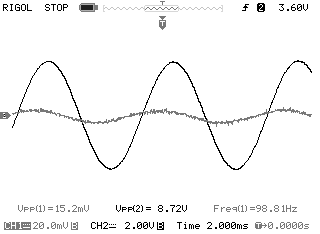
\includegraphics[width=\linewidth]{barrido_100hz.png}\\[-1pt]
{\footnotesize (a) 98,8\,Hz}
\end{minipage}\hfill
\begin{minipage}{0.49\columnwidth}\centering
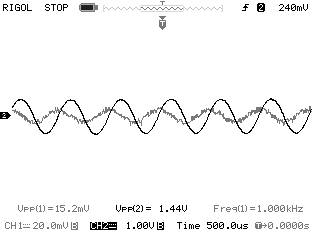
\includegraphics[width=\linewidth]{barrido_1khz.png}\\[-1pt]
{\footnotesize (b) 1\,kHz}
\end{minipage}
\caption{Entrada (CH1, gris) y salida (CH2, negro) durante el barrido. La lectura de Vpp de CH1 está dominada por el ruido. Las capturas se pasaron a escala de grises con fondo blanco para impresión.}
\label{fig:barrido}
\end{figure}

La frecuencia de corte inferior no llegó a medirse. Se intentó determinarla por la respuesta a una onda cuadrada de muy baja frecuencia (constante de tiempo esperada $\tau = RC_3 = 3{,}3$\,s), pero con señales de varios segundos de período el ensayo resultó difícil de capturar con el instrumental disponible y no se completó. El barrido solo permite afirmar que la curva ya es plana a 1\,Hz, lo que con la precisión de la medición ($\pm 0{,}2$\,dB) implica $f_L < 0{,}2$\,Hz. El valor de 0,048\,Hz queda verificado únicamente por cálculo.

%======================================================================
\section{Relación de rechazo de modo común}
\label{sec:rrmc}

Para medir la ganancia de modo común se unieron ambas entradas y se aplicó una senoidal de 50\,Hz, con una amplitud por debajo del umbral de conducción de los diodos de protección. La RRMC se calculó como
\begin{equation}
\text{RRMC} = 20\log\frac{A_{md}(f)}{A_{mc}(f)}, \qquad A_{mc} = \frac{V_{out,mc}}{V_{in,mc}},
\end{equation}
tomando para cada frecuencia la ganancia diferencial del barrido de la Tabla~\ref{tab:barrido}. Las salidas de la primera etapa (512 y 516\,mVpp contra 520\,mVpp de entrada) confirmaron que el modo común la atraviesa con ganancia unitaria, como se espera.

Una primera medición dio una salida de 56 a 59\,mVpp, equivalente a una RRMC de $\approx 79$\,dB. Se tomó con CH2 en 50 y 20\,mV/div y sin promediar, por lo que la lectura estaba inflada por la baja resolución y por el ruido. Al repetirla con CH2 en 10\,mV/div y adquisición promediada, el residuo bajó a 11,6\,mVpp. Además, con el generador conectado y su salida apagada se verificó que la salida no presentaba zumbido apreciable, de modo que el residuo medido corresponde al modo común.

Luego se ajustó RV1 buscando el mínimo de la salida, con lo que el residuo bajó de 11,6 a 6,8\,mVpp (Fig.~\ref{fig:rrmc}). Con RV1 fijo en esa posición, se repitió la medición a otras frecuencias. Los resultados se resumen en la Tabla~\ref{tab:rrmc}.

\begin{figure}[!t]
\centering
\begin{minipage}{0.49\columnwidth}\centering
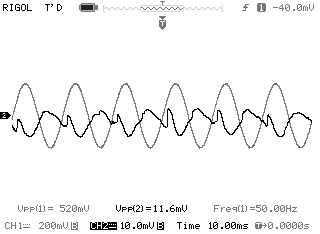
\includegraphics[width=\linewidth]{rrmc_50hz_b_antes_rv1.png}\\[-1pt]
{\footnotesize (a) Antes de ajustar RV1}
\end{minipage}\hfill
\begin{minipage}{0.49\columnwidth}\centering
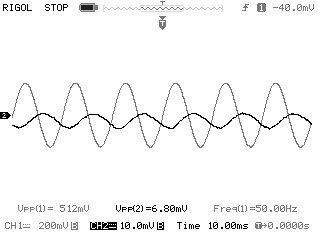
\includegraphics[width=\linewidth]{rrmc_50hz_c_despues_rv1.png}\\[-1pt]
{\footnotesize (b) Después de ajustar RV1}
\end{minipage}
\caption{Ensayo de modo común a 50\,Hz: entrada (CH1, gris, 200\,mV/div) y residuo de salida (CH2, negro, 10\,mV/div).}
\label{fig:rrmc}
\end{figure}

\begin{table}[!t]
\centering
\caption{Rechazo de modo común}
\label{tab:rrmc}
\begin{tabular}{@{}lrrrr@{}}
\toprule
Condición & $f$ (Hz) & $V_{in,mc}$ & $V_{out,mc}$ & RRMC \\
 & & (mVpp) & (mVpp) & (dB) \\ \midrule
Antes de RV1 & 50 & 520 & 11,6 & 92,7 \\
Después de RV1 & 50 & 512 & 6,80 & \textbf{97,2} \\ \midrule
RV1 ajustado & 10 & 480 & 4,20 & $\geq 101{,}7$ \\
RV1 ajustado & 47 & 512 & 6,40 & 97,8 \\
RV1 ajustado & 100 & 528 & 11,2 & 91,9 \\ \bottomrule
\end{tabular}
\end{table}

A 50\,Hz se obtuvo una RRMC de 97,2\,dB, 17\,dB por encima de la especificación. Del análisis de los resultados se desprende que:
\begin{itemize}
\item A 10\,Hz, el residuo no es una senoidal a la frecuencia de excitación sino ruido, por lo que el valor obtenido es una cota inferior.
\item Los resultados a 47 y 50\,Hz son prácticamente iguales, lo que descarta que el zumbido de la red se sumara a la medición a 50\,Hz.
\item La RRMC cae unos 5\,dB entre 50 y 100\,Hz, cerca de los 6\,dB por octava. Esto indica que el desbalance que queda es reactivo. A 50\,Hz la reactancia de C7 y C8 (212\,k$\Omega$) es comparable con las resistencias de 100\,k$\Omega$, de modo que la tolerancia de esos capacitores desbalancea el restador. El trimmer RV1, al ser resistivo, solo puede compensar la componente en fase del desbalance.
\end{itemize}

La simulación confirma esta interpretación (Fig.~\ref{fig:rrmcsim}). Con C7 y C8 idénticos, la RRMC simulada supera los 190\,dB, porque el circuito queda perfectamente balanceado y solo limita el modelo. Con un desbalance de apenas $\delta = 0{,}63$\,\% entre ambos capacitores, la curva simulada pasa por los puntos medidos: a 50\,Hz da $A_{mc} = 0{,}0130$ (medido: 0,0133) y a 100\,Hz, 0,0193 (medido: 0,0212). Con la tolerancia típica de los capacitores de poliéster ($\pm 5$\,\%) la RRMC podría caer por debajo de 80\,dB, por lo que el buen resultado obtenido depende de que C7 y C8 hayan quedado razonablemente apareados.

\begin{figure}[!t]
\centering
\begin{tikzpicture}
\begin{semilogxaxis}[
  width=\columnwidth, height=5.5cm,
  xmin=1, xmax=1000, ymin=50, ymax=140,
  xlabel={$f$ (Hz)}, ylabel={RRMC (dB)},
  xtick={1,10,100,1000}, xticklabels={1,10,100,1k}, ytick distance=10,
  legend style={at={(0.97,0.97)}, anchor=north east, fill=white}]
\addplot[black, thick] table[x=f, y=RRMCdB] {datos/sim_rrmc_dc8_0p63.dat};
\addlegendentry{Sim. $\delta = 0{,}63$\,\%}
\addplot[black, dashed] table[x=f, y=RRMCdB] {datos/sim_rrmc_dc8_2.dat};
\addlegendentry{Sim. $\delta = 2$\,\%}
\addplot[black, dotted, thick] table[x=f, y=RRMCdB] {datos/sim_rrmc_dc8_5.dat};
\addlegendentry{Sim. $\delta = 5$\,\%}
\addplot[black, only marks, mark=o, mark size=2pt, thick] coordinates {(46.95,97.8) (50,97.2) (100,91.9)};
\addlegendentry{Medida}
\addplot[black, only marks, mark=triangle, mark size=2.4pt, thick] coordinates {(10,101.7)};
\addlegendentry{Medida (cota inf.)}
\addplot[gray, dashed] coordinates {(1,80) (1000,80)};
\end{semilogxaxis}
\end{tikzpicture}
\caption{RRMC simulada para distintos desbalances $\delta$ entre C7 y C8, y valores medidos con RV1 ajustado. La línea gris marca la especificación de 80\,dB.}
\label{fig:rrmcsim}
\end{figure}

%======================================================================
\section{Validación con el simulador de ECG}

Por último, se conectó a la placa el simulador de señales biológicas del laboratorio, con LA en la entrada no inversora, RA en la inversora y RL a masa. Con el simulador configurado en ritmo sinusal normal de adulto, 60\,lpm y 1\,mVpp, se obtuvo el trazado de la Fig.~\ref{fig:ecg}(a): un ECG limpio de 1,08\,Vpp, con el complejo QRS hacia arriba, las ondas P y T bien definidas y un intervalo R-R de $\approx 1{,}0$\,s. La ganancia efectiva es de 1080, coherente con la calibración, y no se observa interferencia de 50\,Hz apreciable sobre el trazado.

Como segunda prueba se aumentó la amplitud del simulador a 2\,mVpp con un ritmo más rápido (Fig.~\ref{fig:ecg}(b)). Se obtuvieron 2,02\,Vpp, es decir una ganancia de 1010, y un intervalo R-R de 0,37\,s ($\approx 160$\,lpm, deducido de la propia medición). La morfología se conserva, lo que muestra que el amplificador reproduce correctamente la señal también a mayor amplitud y frecuencia cardíaca.

\begin{figure}[!t]
\centering
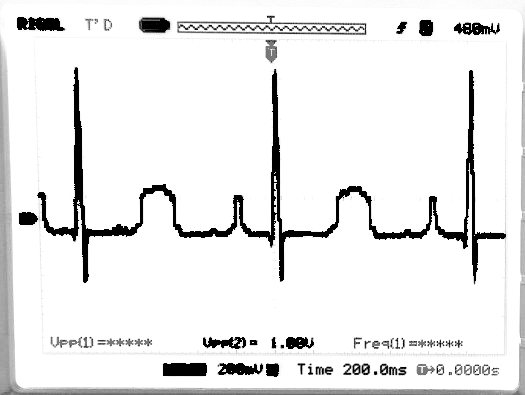
\includegraphics[width=0.68\columnwidth]{ecg_pantalla.jpg}\\[-1pt]
{\footnotesize (a) 1\,mVpp, 60\,lpm (200\,mV/div, 200\,ms/div)}\\[4pt]
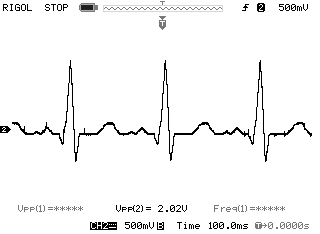
\includegraphics[width=0.54\columnwidth]{ecg2.png}\\[-1pt]
{\footnotesize (b) 2\,mVpp, $\approx 160$\,lpm (500\,mV/div, 100\,ms/div)}
\caption{Salida del amplificador con el simulador de ECG.}
\label{fig:ecg}
\end{figure}

%======================================================================
\section{Conclusiones}

El amplificador cumple las especificaciones verificadas experimentalmente (Tabla~\ref{tab:resumen}). Una vez corregidas las dos fallas de armado (el pad sin soldar en la salida de U1A y el valor erróneo de R11), el circuito alcanzó una ganancia de 60,3\,dB, un ancho de banda superior de 116\,Hz y una RRMC de 97,2\,dB a 50\,Hz. La prueba con el simulador de ECG mostró una señal P-QRS-T limpia, sin necesidad de un filtro de ranura de 50\,Hz que deformaría la señal.

La simulación en LTspice reprodujo las ganancias y las frecuencias de corte de diseño, y además permitió explicar el resultado de RRMC. Con componentes ideales el rechazo supera los 190\,dB; el valor medido corresponde a un desbalance de solo 0,63\,\% entre los capacitores C7 y C8, que RV1 no puede compensar.

\begin{table}[!t]
\centering
\caption{Especificaciones y resultados}
\label{tab:resumen}
\begin{tabular}{@{}llll@{}}
\toprule
Parámetro & Especif. & Simulado & Medido \\ \midrule
$A_{md}$ & 60\,dB & 59,98\,dB & 60,3\,dB \\
$f_H$ & 100\,Hz & 106,2\,Hz & 116\,Hz \\
$f_L$ & 0,05\,Hz & 0,048\,Hz & no medida \\
RRMC (50\,Hz) & $\gg 80$\,dB & 96,9\,dB$^{\ast}$ & 97,2\,dB \\
$Z_i$ & $>5$\,M$\Omega$ & -- & $\sim 10^{12}\,\Omega$$^{\dagger}$ \\
Salida (1\,mVpp) & $\approx 1$\,Vpp & 0,97\,Vpp & 1,08\,Vpp \\ \bottomrule
\multicolumn{4}{@{}l}{\scriptsize $^{\ast}$ con $\delta = 0{,}63$\,\% entre C7 y C8. $^{\dagger}$ según la hoja de datos, no medida.}
\end{tabular}
\end{table}

En cuanto al método, la medición de la RRMC mostró la importancia de la resolución del osciloscopio. La primera medición, hecha con escalas gruesas y sin promediar, subestimaba el rechazo en casi 20\,dB. Del mismo modo, para medir la ganancia con señales de pocos mV conviene usar la punta en $\times 1$ o, como se hizo aquí, inferir la entrada a partir de una etapa de ganancia conocida.

Como mejoras se proponen:
\begin{itemize}
\item aparear C7 y C8, o agregar un ajuste capacitivo, para extender el rechazo de modo común hacia frecuencias más altas;
\item medir $f_L$ con un instrumento de registro lento, por ejemplo un osciloscopio con mayor memoria o una placa de adquisición;
\item reemplazar la etapa de entrada por un amplificador de instrumentación monolítico (por ejemplo INA128 o AD620), cuyas resistencias recortadas por láser permiten superar los 100\,dB de RRMC sin ajustes.
\end{itemize}

%======================================================================
\begin{thebibliography}{4}

\bibitem{ti}
Texas Instruments, ``TL08xx JFET-input operational amplifiers,'' hoja de datos.

\bibitem{catedra}
H.~A. González y P.~G. Miklosa, ``TP3: Aplicaciones lineales de los amplificadores de instrumentación y respuesta en frecuencia,'' Electrónica Aplicada II, UTN FRC.

\bibitem{webster}
J.~G. Webster (Ed.), \emph{Medical Instrumentation: Application and Design}. Hoboken, NJ, USA: Wiley.

\bibitem{pallas}
R.~Pallás-Areny y J.~G. Webster, ``Common mode rejection ratio in differential amplifiers,'' \emph{IEEE Trans. Instrum. Meas.}, vol.~40, no.~4, pp.~669--676, 1991.

\end{thebibliography}

\end{document}
